\section{Решение краевой задачи для дифференциальных уравнений в частных производных эллиптического типа}

\subsection{Постановка задачи}
Решить краевую задачу для дифференциального уравнения эллиптического типа. Аппроксимацию уравнения произвести с использованием центрально-разностной схемы. Для решения дискретного аналога применить следующие методы: метод простых итераций (метод Либмана), метод Зейделя, метод простых итераций с верхней релаксацией. Вычислить погрешность численного решения путем результатов с приведенным в задании аналитическим решением $U(x, y)$ Исследовать зависимость погрешности от сеточных параметров $h_x$, $h_y$.

{\bfseries Вариант:} 8
\begin{align*} 
& \frac{\partial^2 u}{\partial x^2} + \frac{\partial^2 u}{\partial y^2} = -2 \frac{\partial u}{\partial x} - 3 u \\
& u(0, y) = \cos y \\
& u(\frac{\pi}{2}, y) = 0 \\
& u(x, 0) = \exp(-x) \cos x \\
& u(x, \frac{\pi}{2}) = 0 \\
& U(x, y) = \exp(-x) \cos x \cos y \\
\end{align*}
\pagebreak

\subsection{Результаты работы}
\begin{figure}[h!]
\centering
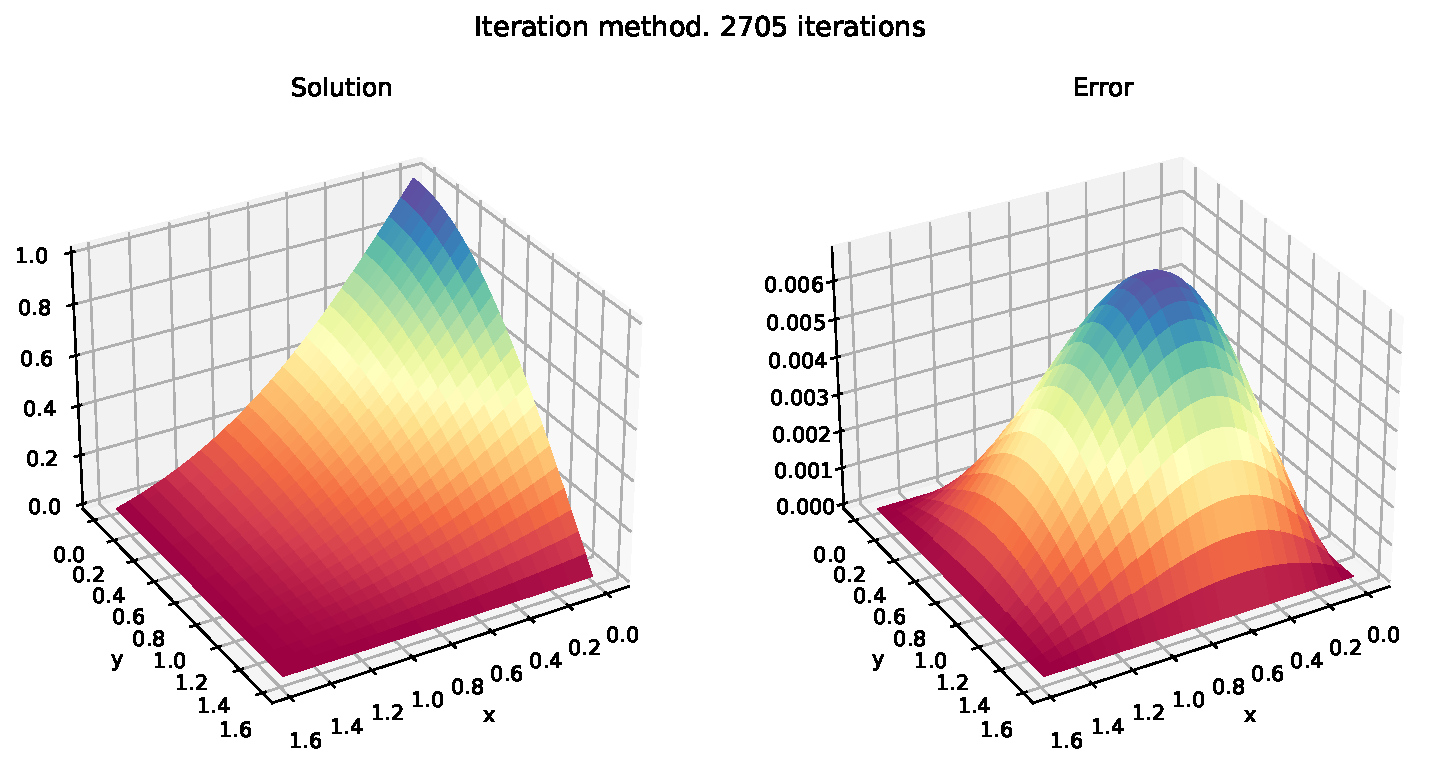
\includegraphics[height=.4\textheight]{lab7_iter}
\caption{Метод простых итераций}
\end{figure}

\vfill

\begin{figure}[h!]
\centering
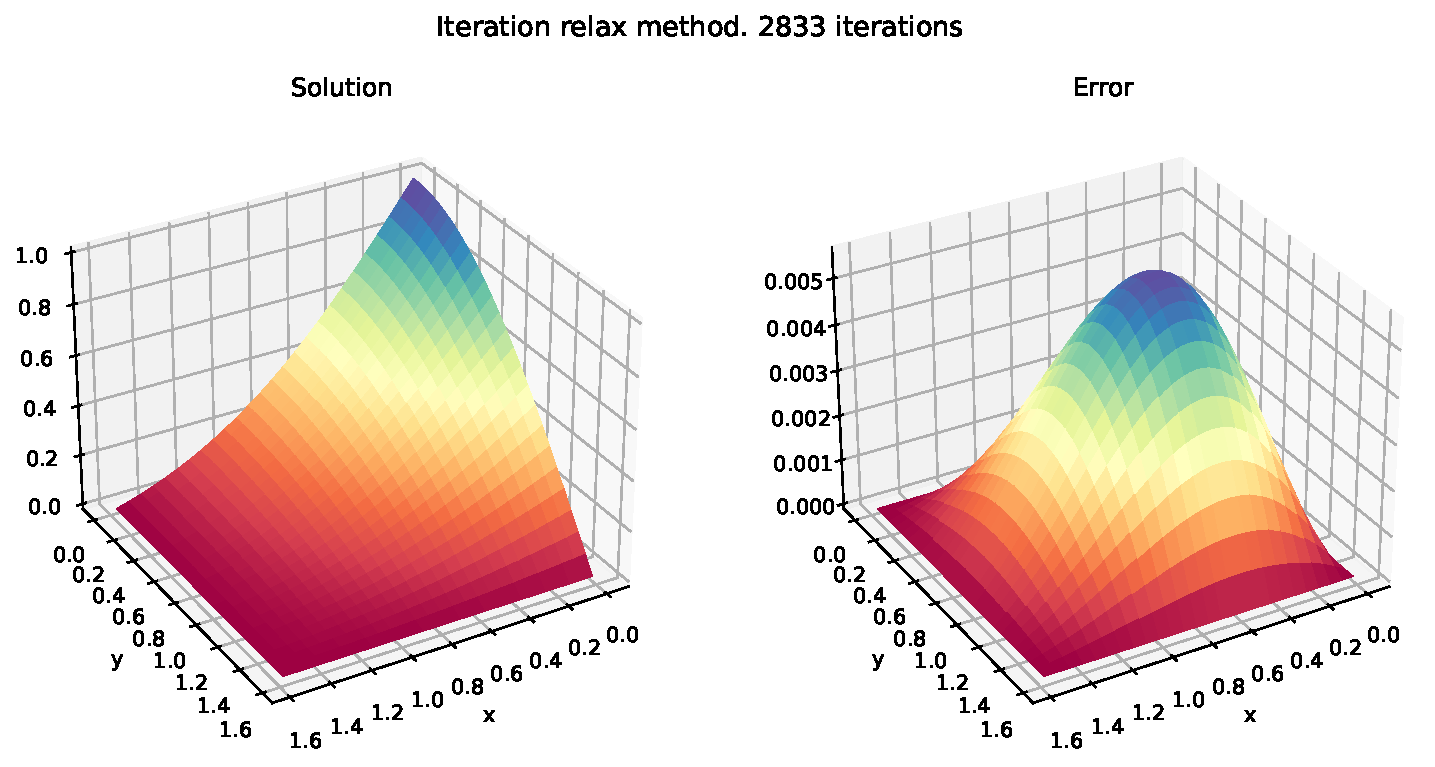
\includegraphics[height=.4\textheight]{lab7_iter_relax}
\caption{Метод простых итераций с верхней релаксацией}
\end{figure}

\pagebreak

\begin{figure}[h!]
\centering
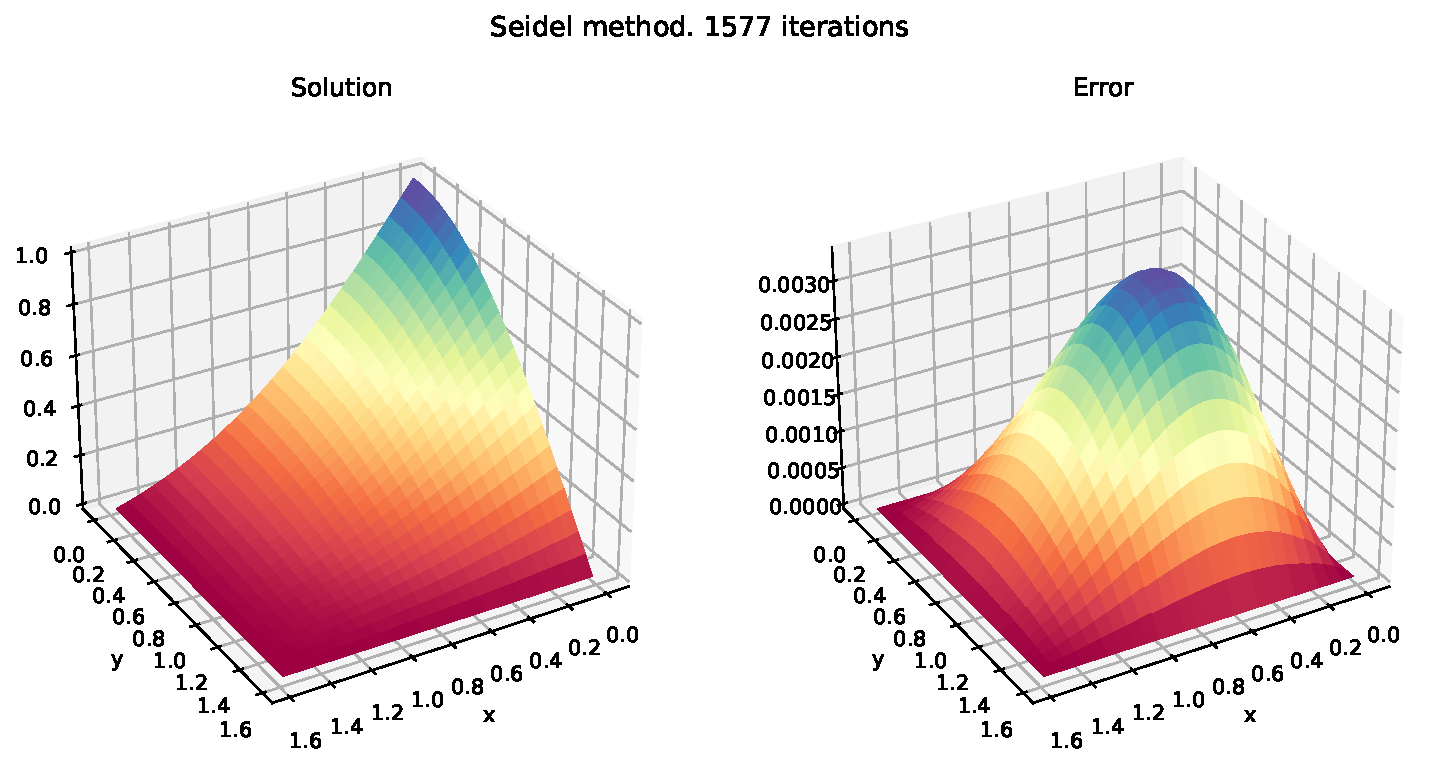
\includegraphics[height=.4\textheight]{lab7_seidel}
\caption{Метод Зейделя}
\end{figure}

\vfill

\begin{figure}[h!]
\centering
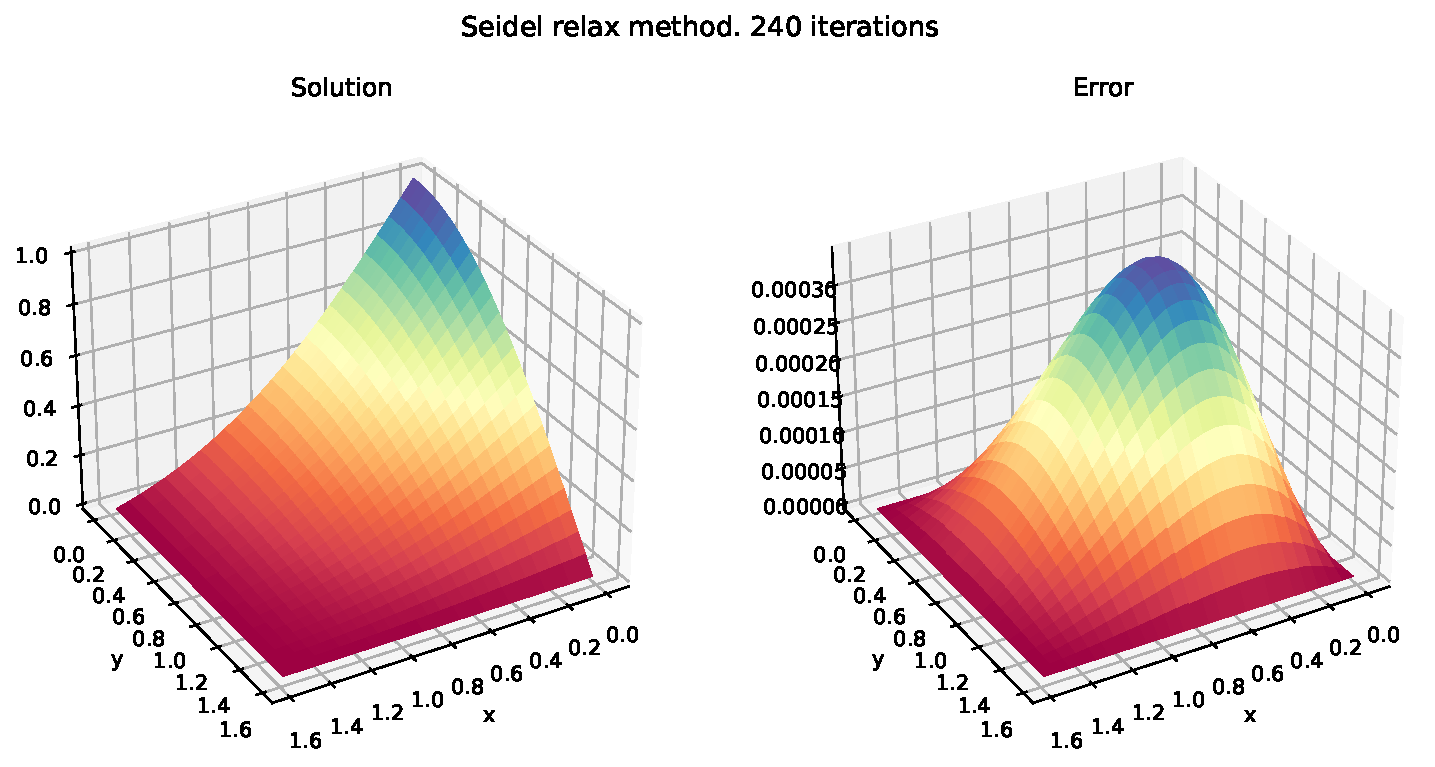
\includegraphics[height=.4\textheight]{lab7_seidel_relax}
\caption{Метод Зейделя с верхней релаксацией}
\end{figure}
\pagebreak

\subsection{Исходный код}
\lstinputlisting{../../include/partial_differential/elliptic_pde.hpp}
\pagebreak
